% Options for packages loaded elsewhere
\PassOptionsToPackage{unicode}{hyperref}
\PassOptionsToPackage{hyphens}{url}
\PassOptionsToPackage{dvipsnames,svgnames,x11names}{xcolor}
%
\documentclass[
  letterpaper,
  DIV=11,
  numbers=noendperiod]{scrartcl}

\usepackage{amsmath,amssymb}
\usepackage{iftex}
\ifPDFTeX
  \usepackage[T1]{fontenc}
  \usepackage[utf8]{inputenc}
  \usepackage{textcomp} % provide euro and other symbols
\else % if luatex or xetex
  \usepackage{unicode-math}
  \defaultfontfeatures{Scale=MatchLowercase}
  \defaultfontfeatures[\rmfamily]{Ligatures=TeX,Scale=1}
\fi
\usepackage{lmodern}
\ifPDFTeX\else  
    % xetex/luatex font selection
\fi
% Use upquote if available, for straight quotes in verbatim environments
\IfFileExists{upquote.sty}{\usepackage{upquote}}{}
\IfFileExists{microtype.sty}{% use microtype if available
  \usepackage[]{microtype}
  \UseMicrotypeSet[protrusion]{basicmath} % disable protrusion for tt fonts
}{}
\makeatletter
\@ifundefined{KOMAClassName}{% if non-KOMA class
  \IfFileExists{parskip.sty}{%
    \usepackage{parskip}
  }{% else
    \setlength{\parindent}{0pt}
    \setlength{\parskip}{6pt plus 2pt minus 1pt}}
}{% if KOMA class
  \KOMAoptions{parskip=half}}
\makeatother
\usepackage{xcolor}
\setlength{\emergencystretch}{3em} % prevent overfull lines
\setcounter{secnumdepth}{5}
% Make \paragraph and \subparagraph free-standing
\ifx\paragraph\undefined\else
  \let\oldparagraph\paragraph
  \renewcommand{\paragraph}[1]{\oldparagraph{#1}\mbox{}}
\fi
\ifx\subparagraph\undefined\else
  \let\oldsubparagraph\subparagraph
  \renewcommand{\subparagraph}[1]{\oldsubparagraph{#1}\mbox{}}
\fi

\usepackage{color}
\usepackage{fancyvrb}
\newcommand{\VerbBar}{|}
\newcommand{\VERB}{\Verb[commandchars=\\\{\}]}
\DefineVerbatimEnvironment{Highlighting}{Verbatim}{commandchars=\\\{\}}
% Add ',fontsize=\small' for more characters per line
\usepackage{framed}
\definecolor{shadecolor}{RGB}{241,243,245}
\newenvironment{Shaded}{\begin{snugshade}}{\end{snugshade}}
\newcommand{\AlertTok}[1]{\textcolor[rgb]{0.68,0.00,0.00}{#1}}
\newcommand{\AnnotationTok}[1]{\textcolor[rgb]{0.37,0.37,0.37}{#1}}
\newcommand{\AttributeTok}[1]{\textcolor[rgb]{0.40,0.45,0.13}{#1}}
\newcommand{\BaseNTok}[1]{\textcolor[rgb]{0.68,0.00,0.00}{#1}}
\newcommand{\BuiltInTok}[1]{\textcolor[rgb]{0.00,0.23,0.31}{#1}}
\newcommand{\CharTok}[1]{\textcolor[rgb]{0.13,0.47,0.30}{#1}}
\newcommand{\CommentTok}[1]{\textcolor[rgb]{0.37,0.37,0.37}{#1}}
\newcommand{\CommentVarTok}[1]{\textcolor[rgb]{0.37,0.37,0.37}{\textit{#1}}}
\newcommand{\ConstantTok}[1]{\textcolor[rgb]{0.56,0.35,0.01}{#1}}
\newcommand{\ControlFlowTok}[1]{\textcolor[rgb]{0.00,0.23,0.31}{#1}}
\newcommand{\DataTypeTok}[1]{\textcolor[rgb]{0.68,0.00,0.00}{#1}}
\newcommand{\DecValTok}[1]{\textcolor[rgb]{0.68,0.00,0.00}{#1}}
\newcommand{\DocumentationTok}[1]{\textcolor[rgb]{0.37,0.37,0.37}{\textit{#1}}}
\newcommand{\ErrorTok}[1]{\textcolor[rgb]{0.68,0.00,0.00}{#1}}
\newcommand{\ExtensionTok}[1]{\textcolor[rgb]{0.00,0.23,0.31}{#1}}
\newcommand{\FloatTok}[1]{\textcolor[rgb]{0.68,0.00,0.00}{#1}}
\newcommand{\FunctionTok}[1]{\textcolor[rgb]{0.28,0.35,0.67}{#1}}
\newcommand{\ImportTok}[1]{\textcolor[rgb]{0.00,0.46,0.62}{#1}}
\newcommand{\InformationTok}[1]{\textcolor[rgb]{0.37,0.37,0.37}{#1}}
\newcommand{\KeywordTok}[1]{\textcolor[rgb]{0.00,0.23,0.31}{#1}}
\newcommand{\NormalTok}[1]{\textcolor[rgb]{0.00,0.23,0.31}{#1}}
\newcommand{\OperatorTok}[1]{\textcolor[rgb]{0.37,0.37,0.37}{#1}}
\newcommand{\OtherTok}[1]{\textcolor[rgb]{0.00,0.23,0.31}{#1}}
\newcommand{\PreprocessorTok}[1]{\textcolor[rgb]{0.68,0.00,0.00}{#1}}
\newcommand{\RegionMarkerTok}[1]{\textcolor[rgb]{0.00,0.23,0.31}{#1}}
\newcommand{\SpecialCharTok}[1]{\textcolor[rgb]{0.37,0.37,0.37}{#1}}
\newcommand{\SpecialStringTok}[1]{\textcolor[rgb]{0.13,0.47,0.30}{#1}}
\newcommand{\StringTok}[1]{\textcolor[rgb]{0.13,0.47,0.30}{#1}}
\newcommand{\VariableTok}[1]{\textcolor[rgb]{0.07,0.07,0.07}{#1}}
\newcommand{\VerbatimStringTok}[1]{\textcolor[rgb]{0.13,0.47,0.30}{#1}}
\newcommand{\WarningTok}[1]{\textcolor[rgb]{0.37,0.37,0.37}{\textit{#1}}}

\providecommand{\tightlist}{%
  \setlength{\itemsep}{0pt}\setlength{\parskip}{0pt}}\usepackage{longtable,booktabs,array}
\usepackage{calc} % for calculating minipage widths
% Correct order of tables after \paragraph or \subparagraph
\usepackage{etoolbox}
\makeatletter
\patchcmd\longtable{\par}{\if@noskipsec\mbox{}\fi\par}{}{}
\makeatother
% Allow footnotes in longtable head/foot
\IfFileExists{footnotehyper.sty}{\usepackage{footnotehyper}}{\usepackage{footnote}}
\makesavenoteenv{longtable}
\usepackage{graphicx}
\makeatletter
\def\maxwidth{\ifdim\Gin@nat@width>\linewidth\linewidth\else\Gin@nat@width\fi}
\def\maxheight{\ifdim\Gin@nat@height>\textheight\textheight\else\Gin@nat@height\fi}
\makeatother
% Scale images if necessary, so that they will not overflow the page
% margins by default, and it is still possible to overwrite the defaults
% using explicit options in \includegraphics[width, height, ...]{}
\setkeys{Gin}{width=\maxwidth,height=\maxheight,keepaspectratio}
% Set default figure placement to htbp
\makeatletter
\def\fps@figure{htbp}
\makeatother

\usepackage{booktabs}
\usepackage{longtable}
\usepackage{array}
\usepackage{multirow}
\usepackage{wrapfig}
\usepackage{float}
\usepackage{colortbl}
\usepackage{pdflscape}
\usepackage{tabu}
\usepackage{threeparttable}
\usepackage{threeparttablex}
\usepackage[normalem]{ulem}
\usepackage{makecell}
\usepackage{xcolor}
\usepackage{tcolorbox}
\tcbuselibrary{breakable}
\tcbset{
  colback=gray!10!white,
  colframe=gray!80!black,
  boxrule=0.4pt,
  arc=4pt,
  left=6pt,
  right=6pt,
  top=6pt,
  bottom=6pt,
  fontupper=\ttfamily\footnotesize
}
\KOMAoption{captions}{tableheading}
\makeatletter
\makeatother
\makeatletter
\makeatother
\makeatletter
\@ifpackageloaded{caption}{}{\usepackage{caption}}
\AtBeginDocument{%
\ifdefined\contentsname
  \renewcommand*\contentsname{Table of contents}
\else
  \newcommand\contentsname{Table of contents}
\fi
\ifdefined\listfigurename
  \renewcommand*\listfigurename{List of Figures}
\else
  \newcommand\listfigurename{List of Figures}
\fi
\ifdefined\listtablename
  \renewcommand*\listtablename{List of Tables}
\else
  \newcommand\listtablename{List of Tables}
\fi
\ifdefined\figurename
  \renewcommand*\figurename{Figure}
\else
  \newcommand\figurename{Figure}
\fi
\ifdefined\tablename
  \renewcommand*\tablename{Table}
\else
  \newcommand\tablename{Table}
\fi
}
\@ifpackageloaded{float}{}{\usepackage{float}}
\floatstyle{ruled}
\@ifundefined{c@chapter}{\newfloat{codelisting}{h}{lop}}{\newfloat{codelisting}{h}{lop}[chapter]}
\floatname{codelisting}{Listing}
\newcommand*\listoflistings{\listof{codelisting}{List of Listings}}
\makeatother
\makeatletter
\@ifpackageloaded{caption}{}{\usepackage{caption}}
\@ifpackageloaded{subcaption}{}{\usepackage{subcaption}}
\makeatother
\makeatletter
\@ifpackageloaded{tcolorbox}{}{\usepackage[skins,breakable]{tcolorbox}}
\makeatother
\makeatletter
\@ifundefined{shadecolor}{\definecolor{shadecolor}{rgb}{.97, .97, .97}}
\makeatother
\makeatletter
\makeatother
\makeatletter
\makeatother
\ifLuaTeX
  \usepackage{selnolig}  % disable illegal ligatures
\fi
\IfFileExists{bookmark.sty}{\usepackage{bookmark}}{\usepackage{hyperref}}
\IfFileExists{xurl.sty}{\usepackage{xurl}}{} % add URL line breaks if available
\urlstyle{same} % disable monospaced font for URLs
\hypersetup{
  pdftitle={Homework 3 - Adv. Macro 1},
  pdfauthor={Davi Jorge},
  colorlinks=true,
  linkcolor={blue},
  filecolor={Maroon},
  citecolor={Blue},
  urlcolor={Blue},
  pdfcreator={LaTeX via pandoc}}

\title{Homework 3 - Adv. Macro 1}
\author{Davi Jorge}
\date{}

\begin{document}
\maketitle
\ifdefined\Shaded\renewenvironment{Shaded}{\begin{tcolorbox}[enhanced, interior hidden, boxrule=0pt, sharp corners, frame hidden, borderline west={3pt}{0pt}{shadecolor}, breakable]}{\end{tcolorbox}}\fi

\renewcommand*\contentsname{Table of contents}
{
\hypersetup{linkcolor=}
\setcounter{tocdepth}{3}
\tableofcontents
}
\hypertarget{homework-4---adv.-macro-1}{%
\section{Homework 4 - Adv. Macro 1}\label{homework-4---adv.-macro-1}}

Link com códigos: \href{https://github.com/davijorge22/adv-macro}{GitHub
-Adv Macro}

\textbf{Questão 1.} De posse da base de dados data\_vec\_alunos.xls,
disponível na pasta da turma, estime um modelo VEC e calcule as
elasticidades de curto e longo prazos da demanda de gasolina.

\begin{itemize}
\tightlist
\item
  \textbf{Aplique a metodologia Engle-Granger como visto em sala de aula
  e compare seus resultados com Alves and Bueno (2003). }
\end{itemize}

\hypertarget{resposta}{%
\subsubsection{Resposta:}\label{resposta}}

\hypertarget{muxe9todo-engle-granger}{%
\paragraph{Método Engle-Granger}\label{muxe9todo-engle-granger}}

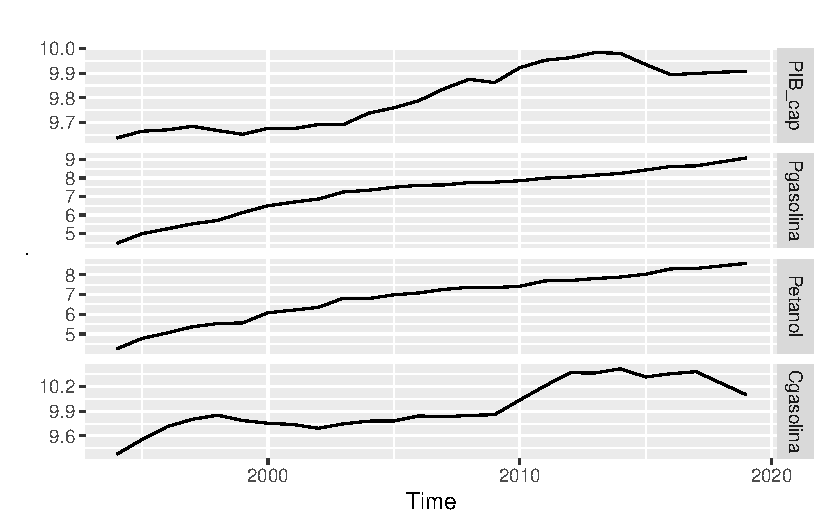
\includegraphics{Homework4_files/figure-pdf/unnamed-chunk-2-1.pdf}

Foi realizado testes de integração nas series e encontrei que as séries
são I(2). Os testes foram feitos a partir do teste de raiz unitária
Dickey Fuller Aumentado.

\begin{verbatim}

Call:
lm(formula = dados_log$Cgasolina ~ t + t2 + dados_log$PIB_cap + 
    dados_log$Pgasolina + dados_log$Petanol)

Residuals:
     Min       1Q   Median       3Q      Max 
-0.23330 -0.03627  0.01522  0.06858  0.20672 

Coefficients:
                     Estimate Std. Error t value Pr(>|t|)  
(Intercept)         13.011827  11.437952   1.138   0.2687  
t                    0.132206   0.110606   1.195   0.2460  
t2                  -0.001884   0.001885  -0.999   0.3295  
dados_log$PIB_cap   -0.233653   1.084191  -0.216   0.8316  
dados_log$Pgasolina -0.776386   0.401886  -1.932   0.0677 .
dados_log$Petanol    0.513779   0.362107   1.419   0.1713  
---
Signif. codes:  0 '***' 0.001 '**' 0.01 '*' 0.05 '.' 0.1 ' ' 1

Residual standard error: 0.127 on 20 degrees of freedom
Multiple R-squared:  0.8484,    Adjusted R-squared:  0.8105 
F-statistic: 22.39 on 5 and 20 DF,  p-value: 0.0000001455
\end{verbatim}

\begin{Shaded}
\begin{Highlighting}[]
\NormalTok{dados\_diff }\OtherTok{=}\NormalTok{ dados\_log }\SpecialCharTok{\%\textgreater{}\%} 
\NormalTok{  dplyr}\SpecialCharTok{::}\FunctionTok{select}\NormalTok{(}\SpecialCharTok{{-}}\NormalTok{Ano) }\SpecialCharTok{\%\textgreater{}\%} 
  \FunctionTok{ts}\NormalTok{(}\AttributeTok{start =} \DecValTok{1994}\NormalTok{) }\SpecialCharTok{\%\textgreater{}\%} 
  \FunctionTok{diff}\NormalTok{(., }\AttributeTok{differences =} \DecValTok{1}\NormalTok{)}


\NormalTok{t }\OtherTok{=} \FunctionTok{c}\NormalTok{(}\DecValTok{1}\SpecialCharTok{:}\FunctionTok{nrow}\NormalTok{(dados\_diff))}
\NormalTok{t2 }\OtherTok{=}\NormalTok{ t}\SpecialCharTok{\^{}}\DecValTok{2}

\NormalTok{ajuste }\OtherTok{\textless{}{-}} \FunctionTok{lm}\NormalTok{(dados\_diff[,}\DecValTok{4}\NormalTok{] }\SpecialCharTok{\textasciitilde{}}\NormalTok{ t }\SpecialCharTok{+}\NormalTok{ t2 }\SpecialCharTok{+}\NormalTok{ dados\_diff[,}\DecValTok{3}\NormalTok{] }\SpecialCharTok{+}\NormalTok{ dados\_diff[,}\DecValTok{2}\NormalTok{] }\SpecialCharTok{+}\NormalTok{ dados\_diff[,}\DecValTok{1}\NormalTok{] }\SpecialCharTok{+}\NormalTok{ cointegracao[}\DecValTok{1}\SpecialCharTok{:}\FunctionTok{nrow}\NormalTok{(dados\_diff)])}

\FunctionTok{summary}\NormalTok{(ajuste)}
\end{Highlighting}
\end{Shaded}

\begin{verbatim}

Call:
lm(formula = dados_diff[, 4] ~ t + t2 + dados_diff[, 3] + dados_diff[, 
    2] + dados_diff[, 1] + cointegracao[1:nrow(dados_diff)])

Residuals:
     Min       1Q   Median       3Q      Max 
-0.11885 -0.04982  0.01168  0.03889  0.10425 

Coefficients:
                                   Estimate Std. Error t value Pr(>|t|)  
(Intercept)                       0.0818915  0.0950404   0.862   0.4009  
t                                 0.0020054  0.0120934   0.166   0.8703  
t2                               -0.0002217  0.0004207  -0.527   0.6050  
dados_diff[, 3]                   0.1776906  0.1447175   1.228   0.2362  
dados_diff[, 2]                  -0.3314786  0.2283426  -1.452   0.1648  
dados_diff[, 1]                  -0.4205767  0.7389193  -0.569   0.5767  
cointegracao[1:nrow(dados_diff)] -0.4033441  0.1509785  -2.672   0.0161 *
---
Signif. codes:  0 '***' 0.001 '**' 0.01 '*' 0.05 '.' 0.1 ' ' 1

Residual standard error: 0.07125 on 17 degrees of freedom
  (1 observation deleted due to missingness)
Multiple R-squared:  0.5201,    Adjusted R-squared:  0.3507 
F-statistic: 3.071 on 6 and 17 DF,  p-value: 0.03184
\end{verbatim}

\newpage

\hypertarget{muxe9todo-johansen}{%
\paragraph{Método Johansen}\label{muxe9todo-johansen}}

\begin{itemize}
\tightlist
\item
  \textbf{Refaça o exercício usando o procedimento de Johansen.}
\end{itemize}

\begin{Shaded}
\begin{Highlighting}[]
\NormalTok{johansen }\OtherTok{\textless{}{-}}\NormalTok{ urca}\SpecialCharTok{::}\FunctionTok{ca.jo}\NormalTok{(dados\_log[,}\SpecialCharTok{{-}}\DecValTok{1}\NormalTok{], }\AttributeTok{type =} \StringTok{\textquotesingle{}trace\textquotesingle{}}\NormalTok{, }\AttributeTok{ecdet =} \StringTok{\textquotesingle{}trend\textquotesingle{}}\NormalTok{, }\AttributeTok{K =} \DecValTok{3}\NormalTok{)}
\FunctionTok{summary}\NormalTok{(johansen)}
\end{Highlighting}
\end{Shaded}

\begin{verbatim}

###################### 
# Johansen-Procedure # 
###################### 

Test type: trace statistic , with linear trend in cointegration 

Eigenvalues (lambda):
[1]  0.9615358873778124815246  0.6475671564918936695676
[3]  0.6002730089127475965327  0.3703585294721342124902
[5] -0.0000000000000001110223

Values of teststatistic and critical values of test:

           test 10pct  5pct  1pct
r <= 3 |  10.64 10.49 12.25 16.26
r <= 2 |  31.73 22.76 25.32 30.45
r <= 1 |  55.72 39.06 42.44 48.45
r = 0  | 130.65 59.14 62.99 70.05

Eigenvectors, normalised to first column:
(These are the cointegration relations)

              PIB_cap.l3 Pgasolina.l3  Petanol.l3 Cgasolina.l3   trend.l3
PIB_cap.l3    1.00000000    1.0000000  1.00000000   1.00000000  1.0000000
Pgasolina.l3  0.97705978   -3.8043676  0.01818656  -0.39309065  1.6840452
Petanol.l3   -1.30244270    6.1368281  0.05575945   0.42015999 -0.2504934
Cgasolina.l3 -0.60147128   -1.5430083 -0.09557703  -0.14476930  2.3076029
trend.l3      0.04512012   -0.2776695 -0.01759161  -0.01934269 -0.3464363

Weights W:
(This is the loading matrix)

            PIB_cap.l3 Pgasolina.l3 Petanol.l3 Cgasolina.l3
PIB_cap.d    0.1876701    0.0582025 -0.2337220   -0.1862419
Pgasolina.d -0.1637809   -0.1363792 -1.7715887    0.5677366
Petanol.d    1.1236732   -0.2576675 -0.4563365    0.1669890
Cgasolina.d  0.9365540    0.1048294  0.3029166    0.3634035
                          trend.l3
PIB_cap.d    0.0000000000001805923
Pgasolina.d -0.0000000000006829817
Petanol.d   -0.0000000000023611743
Cgasolina.d  0.0000000000001828309
\end{verbatim}

\begin{Shaded}
\begin{Highlighting}[]
\FunctionTok{library}\NormalTok{(vars)}
\FunctionTok{VARselect}\NormalTok{(dados\_log[,}\SpecialCharTok{{-}}\DecValTok{1}\NormalTok{], }\AttributeTok{lag.max =} \DecValTok{10}\NormalTok{, }\AttributeTok{type =} \StringTok{"const"}\NormalTok{)}
\end{Highlighting}
\end{Shaded}

\begin{verbatim}
Warning in log(sigma.det): NaNs produzidos
Warning in log(sigma.det): NaNs produzidos
Warning in log(sigma.det): NaNs produzidos
\end{verbatim}

\begin{verbatim}
$selection
AIC(n)  HQ(n)  SC(n) FPE(n) 
     4      4      4      3 

$criteria
                          1                    2
AIC(n) -22.9202396293626016 -22.5862402940521001
HQ(n)  -22.8707860280170365 -22.4972238116300822
SC(n)  -21.9545037265628764 -20.8479156690125933
FPE(n)   0.0000000001211816   0.0000000002805196
                                         3    4    5    6    7    8    9   10
AIC(n)                                 NaN -Inf -Inf -Inf -Inf -Inf -Inf -Inf
HQ(n)                                  NaN -Inf -Inf -Inf -Inf -Inf -Inf -Inf
SC(n)                                  NaN -Inf -Inf -Inf -Inf -Inf -Inf -Inf
FPE(n) -0.00000000000000000000000000457715    0    0    0    0    0    0    0
\end{verbatim}

\begin{Shaded}
\begin{Highlighting}[]
\NormalTok{vec }\OtherTok{\textless{}{-}} \FunctionTok{cajorls}\NormalTok{(johansen, }\AttributeTok{r =} \DecValTok{3}\NormalTok{)  }\CommentTok{\# r = número de vetores cointegrantes, baseado no teste de Johansen}
\FunctionTok{summary}\NormalTok{(vec}\SpecialCharTok{$}\NormalTok{rlm)}
\end{Highlighting}
\end{Shaded}

\begin{verbatim}
Response PIB_cap.d :

Call:
lm(formula = PIB_cap.d ~ ect1 + ect2 + ect3 + constant + PIB_cap.dl1 + 
    Pgasolina.dl1 + Petanol.dl1 + Cgasolina.dl1 + PIB_cap.dl2 + 
    Pgasolina.dl2 + Petanol.dl2 + Cgasolina.dl2 - 1, data = data.mat)

Residuals:
       Min         1Q     Median         3Q        Max 
-0.0301199 -0.0136737  0.0003484  0.0155342  0.0206502 

Coefficients:
               Estimate Std. Error t value Pr(>|t|)
ect1           0.012151   0.204620   0.059    0.954
ect2          -0.042309   0.131709  -0.321    0.754
ect3           0.099717   0.197198   0.506    0.623
constant       1.356363   1.705839   0.795    0.443
PIB_cap.dl1   -0.334846   0.299848  -1.117    0.288
Pgasolina.dl1  0.016659   0.086270   0.193    0.850
Petanol.dl1   -0.015563   0.084654  -0.184    0.857
Cgasolina.dl1  0.009215   0.104150   0.088    0.931
PIB_cap.dl2   -0.266236   0.281529  -0.946    0.365
Pgasolina.dl2  0.024607   0.093208   0.264    0.797
Petanol.dl2    0.015418   0.151960   0.101    0.921
Cgasolina.dl2 -0.065385   0.079243  -0.825    0.427

Residual standard error: 0.02324 on 11 degrees of freedom
Multiple R-squared:  0.6685,    Adjusted R-squared:  0.3069 
F-statistic: 1.849 on 12 and 11 DF,  p-value: 0.1591


Response Pgasolina.d :

Call:
lm(formula = Pgasolina.d ~ ect1 + ect2 + ect3 + constant + PIB_cap.dl1 + 
    Pgasolina.dl1 + Petanol.dl1 + Cgasolina.dl1 + PIB_cap.dl2 + 
    Pgasolina.dl2 + Petanol.dl2 + Cgasolina.dl2 - 1, data = data.mat)

Residuals:
      Min        1Q    Median        3Q       Max 
-0.128731 -0.034478  0.002183  0.038480  0.114321 

Coefficients:
              Estimate Std. Error t value Pr(>|t|)  
ect1           -2.0717     0.7379  -2.808   0.0170 *
ect2            0.3266     0.4750   0.688   0.5059  
ect3           -0.7224     0.7111  -1.016   0.3315  
constant       17.7265     6.1515   2.882   0.0149 *
PIB_cap.dl1    -1.2338     1.0813  -1.141   0.2781  
Pgasolina.dl1  -0.1459     0.3111  -0.469   0.6483  
Petanol.dl1    -0.6383     0.3053  -2.091   0.0605 .
Cgasolina.dl1   0.3707     0.3756   0.987   0.3449  
PIB_cap.dl2    -1.1716     1.0152  -1.154   0.2729  
Pgasolina.dl2   0.1763     0.3361   0.525   0.6102  
Petanol.dl2    -0.8606     0.5480  -1.570   0.1446  
Cgasolina.dl2   0.6218     0.2858   2.176   0.0522 .
---
Signif. codes:  0 '***' 0.001 '**' 0.01 '*' 0.05 '.' 0.1 ' ' 1

Residual standard error: 0.0838 on 11 degrees of freedom
Multiple R-squared:  0.9156,    Adjusted R-squared:  0.8236 
F-statistic: 9.948 on 12 and 11 DF,  p-value: 0.0002957


Response Petanol.d :

Call:
lm(formula = Petanol.d ~ ect1 + ect2 + ect3 + constant + PIB_cap.dl1 + 
    Pgasolina.dl1 + Petanol.dl1 + Cgasolina.dl1 + PIB_cap.dl2 + 
    Pgasolina.dl2 + Petanol.dl2 + Cgasolina.dl2 - 1, data = data.mat)

Residuals:
      Min        1Q    Median        3Q       Max 
-0.098719 -0.020249 -0.000314  0.023334  0.102365 

Coefficients:
              Estimate Std. Error t value  Pr(>|t|)    
ect1            0.4097     0.5168   0.793  0.444684    
ect2            2.0699     0.3326   6.223 0.0000651 ***
ect3           -3.0702     0.4980  -6.165 0.0000706 ***
constant        3.1935     4.3081   0.741  0.474053    
PIB_cap.dl1    -0.3810     0.7573  -0.503  0.624770    
Pgasolina.dl1   0.8237     0.2179   3.781  0.003043 ** 
Petanol.dl1    -1.7481     0.2138  -8.177 0.0000053 ***
Cgasolina.dl1  -0.1735     0.2630  -0.660  0.523093    
PIB_cap.dl2    -2.1084     0.7110  -2.965  0.012850 *  
Pgasolina.dl2   1.1713     0.2354   4.976  0.000418 ***
Petanol.dl2    -2.5352     0.3838  -6.606 0.0000383 ***
Cgasolina.dl2   0.5376     0.2001   2.686  0.021166 *  
---
Signif. codes:  0 '***' 0.001 '**' 0.01 '*' 0.05 '.' 0.1 ' ' 1

Residual standard error: 0.05869 on 11 degrees of freedom
Multiple R-squared:  0.9603,    Adjusted R-squared:  0.9169 
F-statistic: 22.16 on 12 and 11 DF,  p-value: 0.000005729


Response Cgasolina.d :

Call:
lm(formula = Cgasolina.d ~ ect1 + ect2 + ect3 + constant + PIB_cap.dl1 + 
    Pgasolina.dl1 + Petanol.dl1 + Cgasolina.dl1 + PIB_cap.dl2 + 
    Pgasolina.dl2 + Petanol.dl2 + Cgasolina.dl2 - 1, data = data.mat)

Residuals:
      Min        1Q    Median        3Q       Max 
-0.070775 -0.016631 -0.004136  0.027502  0.040881 

Coefficients:
              Estimate Std. Error t value Pr(>|t|)   
ect1           1.34430    0.39837   3.375   0.0062 **
ect2           0.52177    0.25642   2.035   0.0667 . 
ect3          -0.55960    0.38392  -1.458   0.1729   
constant      -5.69600    3.32106  -1.715   0.1143   
PIB_cap.dl1   -1.37895    0.58377  -2.362   0.0377 * 
Pgasolina.dl1  0.27673    0.16796   1.648   0.1277   
Petanol.dl1   -0.15280    0.16481  -0.927   0.3738   
Cgasolina.dl1 -0.04614    0.20277  -0.228   0.8242   
PIB_cap.dl2   -0.35072    0.54810  -0.640   0.5353   
Pgasolina.dl2  0.54440    0.18146   3.000   0.0121 * 
Petanol.dl2   -0.66651    0.29585  -2.253   0.0457 * 
Cgasolina.dl2  0.10318    0.15428   0.669   0.5174   
---
Signif. codes:  0 '***' 0.001 '**' 0.01 '*' 0.05 '.' 0.1 ' ' 1

Residual standard error: 0.04524 on 11 degrees of freedom
Multiple R-squared:  0.8656,    Adjusted R-squared:  0.7189 
F-statistic: 5.902 on 12 and 11 DF,  p-value: 0.003044
\end{verbatim}

\begin{Shaded}
\begin{Highlighting}[]
\NormalTok{vec\_var }\OtherTok{\textless{}{-}} \FunctionTok{vec2var}\NormalTok{(johansen, }\AttributeTok{r =} \DecValTok{3}\NormalTok{)}

\NormalTok{irf\_vec }\OtherTok{\textless{}{-}} \FunctionTok{irf}\NormalTok{(vec\_var,}
               \AttributeTok{runs =} \DecValTok{1000}\NormalTok{,}
               \AttributeTok{impulse =} \StringTok{"Petanol"}\NormalTok{,     }\CommentTok{\# variável que sofre o choque}
              \CommentTok{\# response = "y",    \# variável que responde}
               \AttributeTok{n.ahead =} \DecValTok{20}\NormalTok{,      }\CommentTok{\# horizonte de resposta}
               \AttributeTok{boot =} \ConstantTok{TRUE}\NormalTok{,       }\CommentTok{\# usar bootstrap para intervalo de confiança}
               \AttributeTok{ci =} \FloatTok{0.95}\NormalTok{,}
\NormalTok{               )         }\CommentTok{\# intervalo de 95\%}

\FunctionTok{plot}\NormalTok{(irf\_vec)}
\end{Highlighting}
\end{Shaded}

\begin{figure}[H]

{\centering 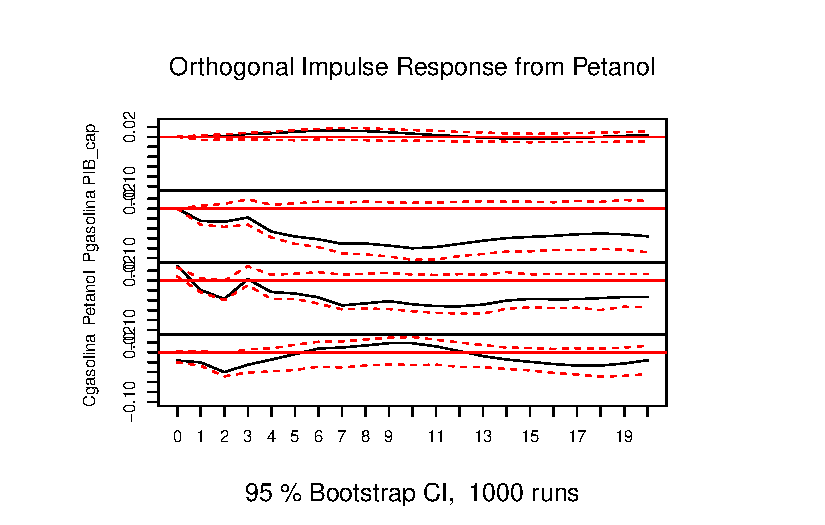
\includegraphics{Homework4_files/figure-pdf/unnamed-chunk-5-1.pdf}

}

\end{figure}

\textbf{Questão 2.} De posse da base de dados quartely.xls, disponível
na pasta da turma, estime um modelo VEC para a relação entre a Tbill e a
Tbill\_3year replicando os resultados de sala de aula.

\begin{itemize}
\tightlist
\item
  \textbf{Aplique a metodologia Engle-Granger e o procedimento de
  Johansen separadamente. Você deve apresentar a relação de longo prazo
  estimada.}
\end{itemize}

\hypertarget{resposta-1}{%
\subsubsection{Resposta:}\label{resposta-1}}

\hypertarget{muxe9todo-engle-granger-1}{%
\paragraph{Método Engle-Granger}\label{muxe9todo-engle-granger-1}}

\begin{Shaded}
\begin{Highlighting}[]
\NormalTok{dados\_vec2 }\OtherTok{=} \FunctionTok{tibble}\NormalTok{(}
  \AttributeTok{tbill =}\NormalTok{ dados}\SpecialCharTok{$}\NormalTok{tbill }\SpecialCharTok{\%\textgreater{}\%} \FunctionTok{diff}\NormalTok{(),}
  \AttributeTok{tbill\_3year =}\NormalTok{ dados}\SpecialCharTok{$}\NormalTok{tbill\_3year }\SpecialCharTok{\%\textgreater{}\%} \FunctionTok{diff}\NormalTok{(),}
  \AttributeTok{coef\_lp =}\NormalTok{ cointegracao[}\SpecialCharTok{{-}}\DecValTok{1}\NormalTok{])}

\NormalTok{dados\_vec2 }\OtherTok{=} \FunctionTok{tibble}\NormalTok{(}
  \AttributeTok{tbill =}\NormalTok{ dados}\SpecialCharTok{$}\NormalTok{tbill,}
  \AttributeTok{tbill\_3year =}\NormalTok{ dados}\SpecialCharTok{$}\NormalTok{tbill\_3year,}
  \AttributeTok{coef\_lp =}\NormalTok{ cointegracao) }\SpecialCharTok{\%\textgreater{}\%} 
  \FunctionTok{na.omit}\NormalTok{()}


\NormalTok{vars}\SpecialCharTok{::}\FunctionTok{VARselect}\NormalTok{(dados\_vec2, }\AttributeTok{type =} \StringTok{\textquotesingle{}none\textquotesingle{}}\NormalTok{)}
\end{Highlighting}
\end{Shaded}

\begin{verbatim}
$selection
AIC(n)  HQ(n)  SC(n) FPE(n) 
     6      2      2      6 

$criteria
                  1                                         2
AIC(n) -5.478585902 -71.0256107937762664050751482136547565460
HQ(n)  -5.414356676 -70.8971523407930703797319438308477401733
SC(n)  -5.320146011 -70.7087310115379068520269356667995452881
FPE(n)  0.004175267   0.0000000000000000000000000000001425609
                                               3
AIC(n) -71.0121764811915596737890155054628849030
HQ(n)  -70.8194888017167585303468513302505016327
SC(n)  -70.5368568078340132387893390841782093048
FPE(n)   0.0000000000000000000000000000001445136
                                               4
AIC(n) -71.0114720678783299945280305109918117523
HQ(n)  -70.7545551619119237329869065433740615845
SC(n)  -70.3777125034015966775768902152776718140
FPE(n)   0.0000000000000000000000000000001446636
                                              5
AIC(n) -71.035879659942651187520823441445827484
HQ(n)  -70.714733527484639807880739681422710419
SC(n)  -70.243680204346730988618219271302223206
FPE(n)   0.000000000000000000000000000000141253
                                               6
AIC(n) -71.1061983113538360612437827512621879578
HQ(n)  -70.7208229524042479852141696028411388397
SC(n)  -70.1555589646387431912444299086928367615
FPE(n)   0.0000000000000000000000000000001317697
                                               7
AIC(n) -71.0293476850461047433782368898391723633
HQ(n)  -70.5797430996049115492496639490127563477
SC(n)  -69.9202684472118249914274201728403568268
FPE(n)   0.0000000000000000000000000000001424595
                                               8
AIC(n) -71.0174097692510457591197337023913860321
HQ(n)  -70.5035759573182474468922009691596031189
SC(n)  -69.7498906402975791252174531109631061554
FPE(n)   0.0000000000000000000000000000001443922
                                               9
AIC(n) -70.9873595765837990256841294467449188232
HQ(n)  -70.4092965381593955953576369211077690125
SC(n)  -69.5614005565111597206851001828908920288
FPE(n)   0.0000000000000000000000000000001490924
                                              10
AIC(n) -70.9191987798172931434237398207187652588
HQ(n)  -70.2769065149012988058530027046799659729
SC(n)  -69.3347998686254811673279618844389915466
FPE(n)   0.0000000000000000000000000000001600067
\end{verbatim}

\begin{Shaded}
\begin{Highlighting}[]
\NormalTok{vars}\SpecialCharTok{::}\FunctionTok{VAR}\NormalTok{(dados\_vec2, }\AttributeTok{p =} \DecValTok{8}\NormalTok{, }\AttributeTok{type =} \StringTok{\textquotesingle{}none\textquotesingle{}}\NormalTok{)}
\end{Highlighting}
\end{Shaded}

\begin{verbatim}

VAR Estimation Results:
======================= 

Estimated coefficients for equation tbill: 
========================================== 
Call:
tbill = tbill.l1 + tbill_3year.l1 + coef_lp.l1 + tbill.l2 + tbill_3year.l2 + coef_lp.l2 + tbill.l3 + tbill_3year.l3 + coef_lp.l3 + tbill.l4 + tbill_3year.l4 + coef_lp.l4 + tbill.l5 + tbill_3year.l5 + coef_lp.l5 + tbill.l6 + tbill_3year.l6 + coef_lp.l6 + tbill.l7 + tbill_3year.l7 + coef_lp.l7 + tbill.l8 + tbill_3year.l8 + coef_lp.l8 

      tbill.l1 tbill_3year.l1     coef_lp.l1       tbill.l2 tbill_3year.l2 
   1.164965868    0.266810781    0.403413847   -0.871332367    0.009275775 
    coef_lp.l2       tbill.l3 tbill_3year.l3     coef_lp.l3       tbill.l4 
  -0.263495646    0.767379346             NA    0.035473219   -0.438241685 
tbill_3year.l4     coef_lp.l4       tbill.l5 tbill_3year.l5     coef_lp.l5 
            NA    0.253464376    0.175778300             NA   -0.427784260 
      tbill.l6 tbill_3year.l6     coef_lp.l6       tbill.l7 tbill_3year.l7 
  -0.109267884             NA    0.266606481   -0.220218111             NA 
    coef_lp.l7       tbill.l8 tbill_3year.l8     coef_lp.l8 
  -0.090292300    0.206775161             NA   -0.022637437 


Estimated coefficients for equation tbill_3year: 
================================================ 
Call:
tbill_3year = tbill.l1 + tbill_3year.l1 + coef_lp.l1 + tbill.l2 + tbill_3year.l2 + coef_lp.l2 + tbill.l3 + tbill_3year.l3 + coef_lp.l3 + tbill.l4 + tbill_3year.l4 + coef_lp.l4 + tbill.l5 + tbill_3year.l5 + coef_lp.l5 + tbill.l6 + tbill_3year.l6 + coef_lp.l6 + tbill.l7 + tbill_3year.l7 + coef_lp.l7 + tbill.l8 + tbill_3year.l8 + coef_lp.l8 

      tbill.l1 tbill_3year.l1     coef_lp.l1       tbill.l2 tbill_3year.l2 
   0.116943752    1.128651109    0.449193105   -0.511151637   -0.016931162 
    coef_lp.l2       tbill.l3 tbill_3year.l3     coef_lp.l3       tbill.l4 
  -0.335044880    0.527114586             NA    0.191688453   -0.336417230 
tbill_3year.l4     coef_lp.l4       tbill.l5 tbill_3year.l5     coef_lp.l5 
            NA    0.276906250    0.022564458             NA   -0.248425446 
      tbill.l6 tbill_3year.l6     coef_lp.l6       tbill.l7 tbill_3year.l7 
   0.000161308             NA    0.057006330   -0.159333241             NA 
    coef_lp.l7       tbill.l8 tbill_3year.l8     coef_lp.l8 
  -0.299590374    0.207867502             NA    0.166036857 


Estimated coefficients for equation coef_lp: 
============================================ 
Call:
coef_lp = tbill.l1 + tbill_3year.l1 + coef_lp.l1 + tbill.l2 + tbill_3year.l2 + coef_lp.l2 + tbill.l3 + tbill_3year.l3 + coef_lp.l3 + tbill.l4 + tbill_3year.l4 + coef_lp.l4 + tbill.l5 + tbill_3year.l5 + coef_lp.l5 + tbill.l6 + tbill_3year.l6 + coef_lp.l6 + tbill.l7 + tbill_3year.l7 + coef_lp.l7 + tbill.l8 + tbill_3year.l8 + coef_lp.l8 

                  tbill.l1             tbill_3year.l1 
 0.99999999999999911182158 -0.95815229211599028946722 
                coef_lp.l1                   tbill.l2 
 0.99999999999999911182158 -0.99999999999999977795540 
            tbill_3year.l2                 coef_lp.l2 
 0.95815229211599028946722  0.00000000000000088139872 
                  tbill.l3             tbill_3year.l3 
 0.00000000000000010961856                         NA 
                coef_lp.l3                   tbill.l4 
-0.00000000000000089374087 -0.00000000000000008267233 
            tbill_3year.l4                 coef_lp.l4 
                        NA -0.00000000000000017055803 
                  tbill.l5             tbill_3year.l5 
 0.00000000000000037650921                         NA 
                coef_lp.l5                   tbill.l6 
 0.00000000000000015625905 -0.00000000000000020337856 
            tbill_3year.l6                 coef_lp.l6 
                        NA -0.00000000000000082517915 
                  tbill.l7             tbill_3year.l7 
 0.00000000000000059033412                         NA 
                coef_lp.l7                   tbill.l8 
 0.00000000000000140660912 -0.00000000000000055748310 
            tbill_3year.l8                 coef_lp.l8 
                        NA -0.00000000000000089729162 
\end{verbatim}

\newpage

\hypertarget{muxe9todo-johansen-1}{%
\paragraph{Método Johansen}\label{muxe9todo-johansen-1}}

\begin{itemize}
\tightlist
\item
  \textbf{Refaça o exercício usando o procedimento de Johansen.}
\end{itemize}

\begin{Shaded}
\begin{Highlighting}[]
\NormalTok{johansen }\OtherTok{\textless{}{-}}\NormalTok{ urca}\SpecialCharTok{::}\FunctionTok{ca.jo}\NormalTok{(dados[,}\FunctionTok{c}\NormalTok{(}\DecValTok{3}\NormalTok{,}\DecValTok{4}\NormalTok{)], }\AttributeTok{type =} \StringTok{\textquotesingle{}trace\textquotesingle{}}\NormalTok{, }\AttributeTok{ecdet =} \StringTok{\textquotesingle{}const\textquotesingle{}}\NormalTok{, }\AttributeTok{K =} \DecValTok{7}\NormalTok{)}
\FunctionTok{summary}\NormalTok{(johansen)}
\end{Highlighting}
\end{Shaded}

\begin{verbatim}

###################### 
# Johansen-Procedure # 
###################### 

Test type: trace statistic , without linear trend and constant in cointegration 

Eigenvalues (lambda):
[1] 0.136776622128432112646124 0.007857000246084197558893
[3] 0.000000000000000002385245

Values of teststatistic and critical values of test:

          test 10pct  5pct  1pct
r <= 1 |  1.47  7.52  9.24 12.97
r = 0  | 28.82 17.85 19.96 24.60

Eigenvectors, normalised to first column:
(These are the cointegration relations)

                  tbill.l7 tbill_3year.l7  constant
tbill.l7        1.00000000       1.000000  1.000000
tbill_3year.l7 -0.86851862      -1.452007 -1.240983
constant        0.07842768       3.583613  5.689802

Weights W:
(This is the loading matrix)

                 tbill.l7 tbill_3year.l7                   constant
tbill.d       -0.28232732     0.03307991 -0.00000000000000001887690
tbill_3year.d -0.02224397     0.03730258 -0.00000000000000007082296
\end{verbatim}

\begin{Shaded}
\begin{Highlighting}[]
\FunctionTok{library}\NormalTok{(vars)}
\FunctionTok{VARselect}\NormalTok{(dados[,}\FunctionTok{c}\NormalTok{(}\DecValTok{3}\NormalTok{,}\DecValTok{4}\NormalTok{)], }\AttributeTok{lag.max =} \DecValTok{10}\NormalTok{, }\AttributeTok{type =} \StringTok{"const"}\NormalTok{)}
\end{Highlighting}
\end{Shaded}

\begin{verbatim}
$selection
AIC(n)  HQ(n)  SC(n) FPE(n) 
     9      7      2      9 

$criteria
                 1           2           3           4           5           6
AIC(n) -2.49011733 -2.58479975 -2.59495858 -2.66192876 -2.63340749 -2.76319343
HQ(n)  -2.44746282 -2.51370890 -2.49543139 -2.53396524 -2.47700763 -2.57835723
SC(n)  -2.38488827 -2.40941799 -2.34942412 -2.34624159 -2.24756762 -2.30720086
FPE(n)  0.08290073  0.07541323  0.07465454  0.06982453  0.07185412  0.06312023
                 7           8           9          10
AIC(n) -2.79605824 -2.79143757 -2.83461341 -2.82020086
HQ(n)  -2.58278571 -2.54972870 -2.56446820 -2.52161932
SC(n)  -2.26991297 -2.19513959 -2.16816274 -2.08359748
FPE(n)  0.06109526  0.06139892  0.05882953  0.05971513
\end{verbatim}

\begin{Shaded}
\begin{Highlighting}[]
\NormalTok{vec }\OtherTok{\textless{}{-}} \FunctionTok{cajorls}\NormalTok{(johansen, }\AttributeTok{r =} \DecValTok{1}\NormalTok{)  }\CommentTok{\# r = número de vetores cointegrantes, baseado no teste de Johansen}
\FunctionTok{summary}\NormalTok{(vec}\SpecialCharTok{$}\NormalTok{rlm)}
\end{Highlighting}
\end{Shaded}

\begin{verbatim}
Response tbill.d :

Call:
lm(formula = tbill.d ~ ect1 + tbill.dl1 + tbill_3year.dl1 + tbill.dl2 + 
    tbill_3year.dl2 + tbill.dl3 + tbill_3year.dl3 + tbill.dl4 + 
    tbill_3year.dl4 + tbill.dl5 + tbill_3year.dl5 + tbill.dl6 + 
    tbill_3year.dl6 - 1, data = data.mat)

Residuals:
     Min       1Q   Median       3Q      Max 
-2.99145 -0.28876 -0.00276  0.25416  3.15640 

Coefficients:
                 Estimate Std. Error t value Pr(>|t|)    
ect1            -0.282327   0.092262  -3.060 0.002566 ** 
tbill.dl1        0.153794   0.135100   1.138 0.256537    
tbill_3year.dl1  0.299049   0.148218   2.018 0.045176 *  
tbill.dl2       -0.413591   0.128007  -3.231 0.001477 ** 
tbill_3year.dl2 -0.003426   0.145009  -0.024 0.981176    
tbill.dl3        0.175233   0.139260   1.258 0.209972    
tbill_3year.dl3  0.220790   0.148432   1.487 0.138708    
tbill.dl4       -0.312628   0.131899  -2.370 0.018879 *  
tbill_3year.dl4  0.168718   0.148750   1.134 0.258264    
tbill.dl5        0.246904   0.137059   1.801 0.073375 .  
tbill_3year.dl5 -0.073751   0.151894  -0.486 0.627907    
tbill.dl6       -0.447088   0.130269  -3.432 0.000749 ***
tbill_3year.dl6  0.364868   0.156638   2.329 0.020995 *  
---
Signif. codes:  0 '***' 0.001 '**' 0.01 '*' 0.05 '.' 0.1 ' ' 1

Residual standard error: 0.6698 on 173 degrees of freedom
Multiple R-squared:  0.3031,    Adjusted R-squared:  0.2508 
F-statistic: 5.789 on 13 and 173 DF,  p-value: 0.00000000848


Response tbill_3year.d :

Call:
lm(formula = tbill_3year.d ~ ect1 + tbill.dl1 + tbill_3year.dl1 + 
    tbill.dl2 + tbill_3year.dl2 + tbill.dl3 + tbill_3year.dl3 + 
    tbill.dl4 + tbill_3year.dl4 + tbill.dl5 + tbill_3year.dl5 + 
    tbill.dl6 + tbill_3year.dl6 - 1, data = data.mat)

Residuals:
     Min       1Q   Median       3Q      Max 
-2.63052 -0.31921  0.01428  0.32392  1.61584 

Coefficients:
                 Estimate Std. Error t value Pr(>|t|)   
ect1            -0.022244   0.084527  -0.263  0.79274   
tbill.dl1        0.103963   0.123772   0.840  0.40209   
tbill_3year.dl1  0.168927   0.135791   1.244  0.21517   
tbill.dl2       -0.006436   0.117274  -0.055  0.95630   
tbill_3year.dl2 -0.260350   0.132851  -1.960  0.05164 . 
tbill.dl3        0.190904   0.127583   1.496  0.13640   
tbill_3year.dl3  0.075421   0.135987   0.555  0.57987   
tbill.dl4        0.007899   0.120839   0.065  0.94796   
tbill_3year.dl4 -0.121484   0.136278  -0.891  0.37393   
tbill.dl5        0.382903   0.125567   3.049  0.00265 **
tbill_3year.dl5 -0.360911   0.139158  -2.594  0.01031 * 
tbill.dl6        0.047190   0.119346   0.395  0.69303   
tbill_3year.dl6 -0.135400   0.143504  -0.944  0.34673   
---
Signif. codes:  0 '***' 0.001 '**' 0.01 '*' 0.05 '.' 0.1 ' ' 1

Residual standard error: 0.6136 on 173 degrees of freedom
Multiple R-squared:  0.203, Adjusted R-squared:  0.1432 
F-statistic:  3.39 on 13 and 173 DF,  p-value: 0.0001157
\end{verbatim}

\begin{Shaded}
\begin{Highlighting}[]
\NormalTok{vec\_var }\OtherTok{\textless{}{-}} \FunctionTok{vec2var}\NormalTok{(johansen, }\AttributeTok{r =} \DecValTok{1}\NormalTok{)}

\NormalTok{irf\_vec }\OtherTok{\textless{}{-}} \FunctionTok{irf}\NormalTok{(vec\_var,}
               \AttributeTok{runs =} \DecValTok{1000}\NormalTok{,}
               \CommentTok{\#impulse = "Petanol",     \# variável que sofre o choque}
              \CommentTok{\# response = "y",    \# variável que responde}
               \AttributeTok{n.ahead =} \DecValTok{20}\NormalTok{,      }\CommentTok{\# horizonte de resposta}
               \AttributeTok{boot =} \ConstantTok{TRUE}\NormalTok{,       }\CommentTok{\# usar bootstrap para intervalo de confiança}
               \AttributeTok{ci =} \FloatTok{0.95}\NormalTok{,}
\NormalTok{               )         }\CommentTok{\# intervalo de 95\%}

\FunctionTok{plot}\NormalTok{(irf\_vec)}
\end{Highlighting}
\end{Shaded}

\begin{figure}[H]

{\centering 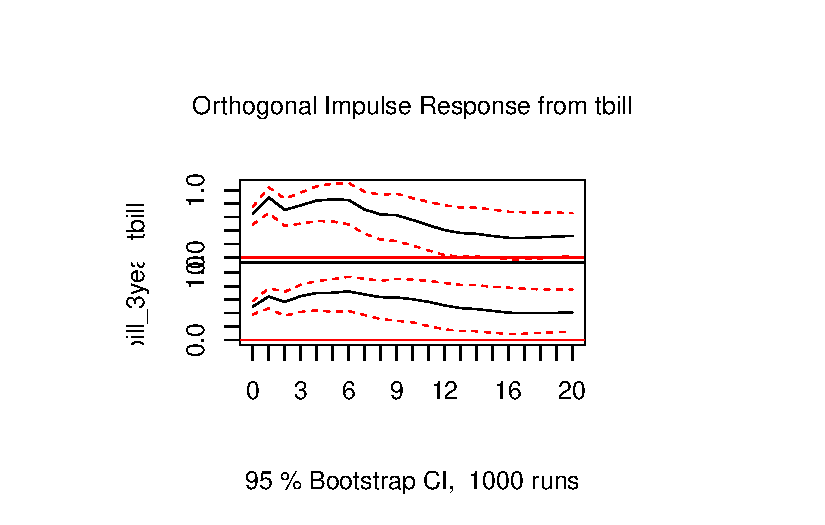
\includegraphics{Homework4_files/figure-pdf/unnamed-chunk-9-1.pdf}

}

\end{figure}

\begin{figure}[H]

{\centering 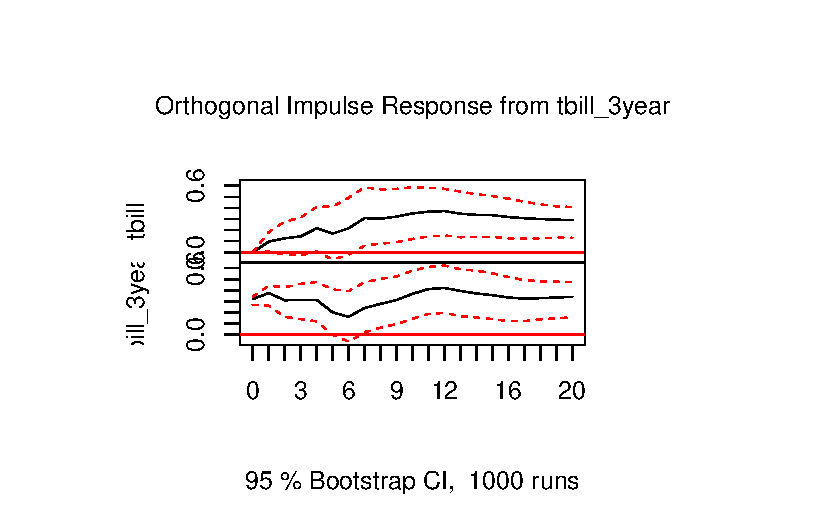
\includegraphics{Homework4_files/figure-pdf/unnamed-chunk-9-2.pdf}

}

\end{figure}



\end{document}
